\sectionmark{MEX 3-1: CNL Test}
\section[MEX 3-1: CNL direct shear test]{Model-Experiment-Exercise MEX 3-1:\\Constant normal load (CNL) direct shear test}
\sectionmark{MEX 3-1: CNL Test}% using this twice is not nice style...
\label{sec:mex07}\index{Constant Normal Load (CNL) experiment}
%\index{CNL Constant Normal Load test}
%------------------------------------------------------------------------------
\Authors{Daniel P\"otschke, Thomas Fr\"uhwirt}
%------------------------------------------------------------------------------
\subsection{Experimental set-up}
%------------------------------------------------------------------------------
\begin{figure}[!ht]
\begin{center}
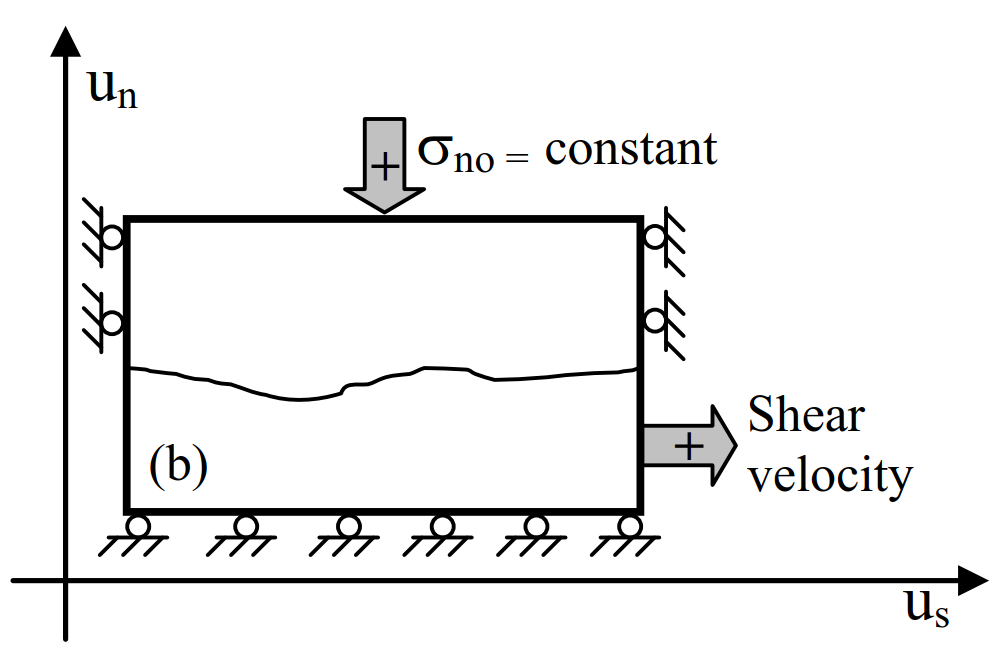
\includegraphics[width=0.5\textwidth]{./figures/MEX7_CNL_Nguyen_Thesis.PNG}
\end{center}
\caption{Constant normal load (CNL) direct shear test. (From: \cite{Nguyen2014})}
\label{fig:MEX7_CNL}
\end{figure}
Direct shear tests are conducted in rock mechanical laboratories to investigate the shear characteristics of rock fractures/joints. The samples are blocks or cylin\-ders which are separated in two parts by a fracture. This fracture can be a natural one or an artificial one. Artificial fractures can be created by shearing of the intact sample or by a Brazilian test.
%
A schematic illustration of direct shear test can be seen in Figure \ref{fig:MEX7_CNL}. During a direct shear test a normal force acts on the rock fracture. One part of the sample is fixed and the other one is sheared against it. The shear forces are measured while the two parts are separated against each other at a specific shear rate.
\index{Brazilian test}

In this model exercise a constant normal load (CNL) boundary condition has been applied. This means the normal stress acting on the fracture remains constant during the shear displacement. An analogy in the nature would be a rock boulder at a slope or a dam where in both cases the self weight of the top part creates the normal stress at the contact region/fracture.
%
A rock fracture in nature is usually rough at some degree of detail. In the direct shear tests the two parts of the sample fit more or less perfectly at the initial position. The fracture is closed. When they are sheared against each other the unevenness, the roughness, causes an opening of the fracture and an uplift of the upper part. This so called normal displacement or dilatation is free like the rock boulder on the slope could easily uplift as only his constant weight is acting on it.

The experimental procedure involves a surface scan of the rock fracture as a first step. This geometric information are used to determine the roughness of the surface. The output of the scanning device is a point cloud, as seen in Figure \ref{fig:MEX7_pointCloud}.

\begin{figure}[!ht]
\begin{center}
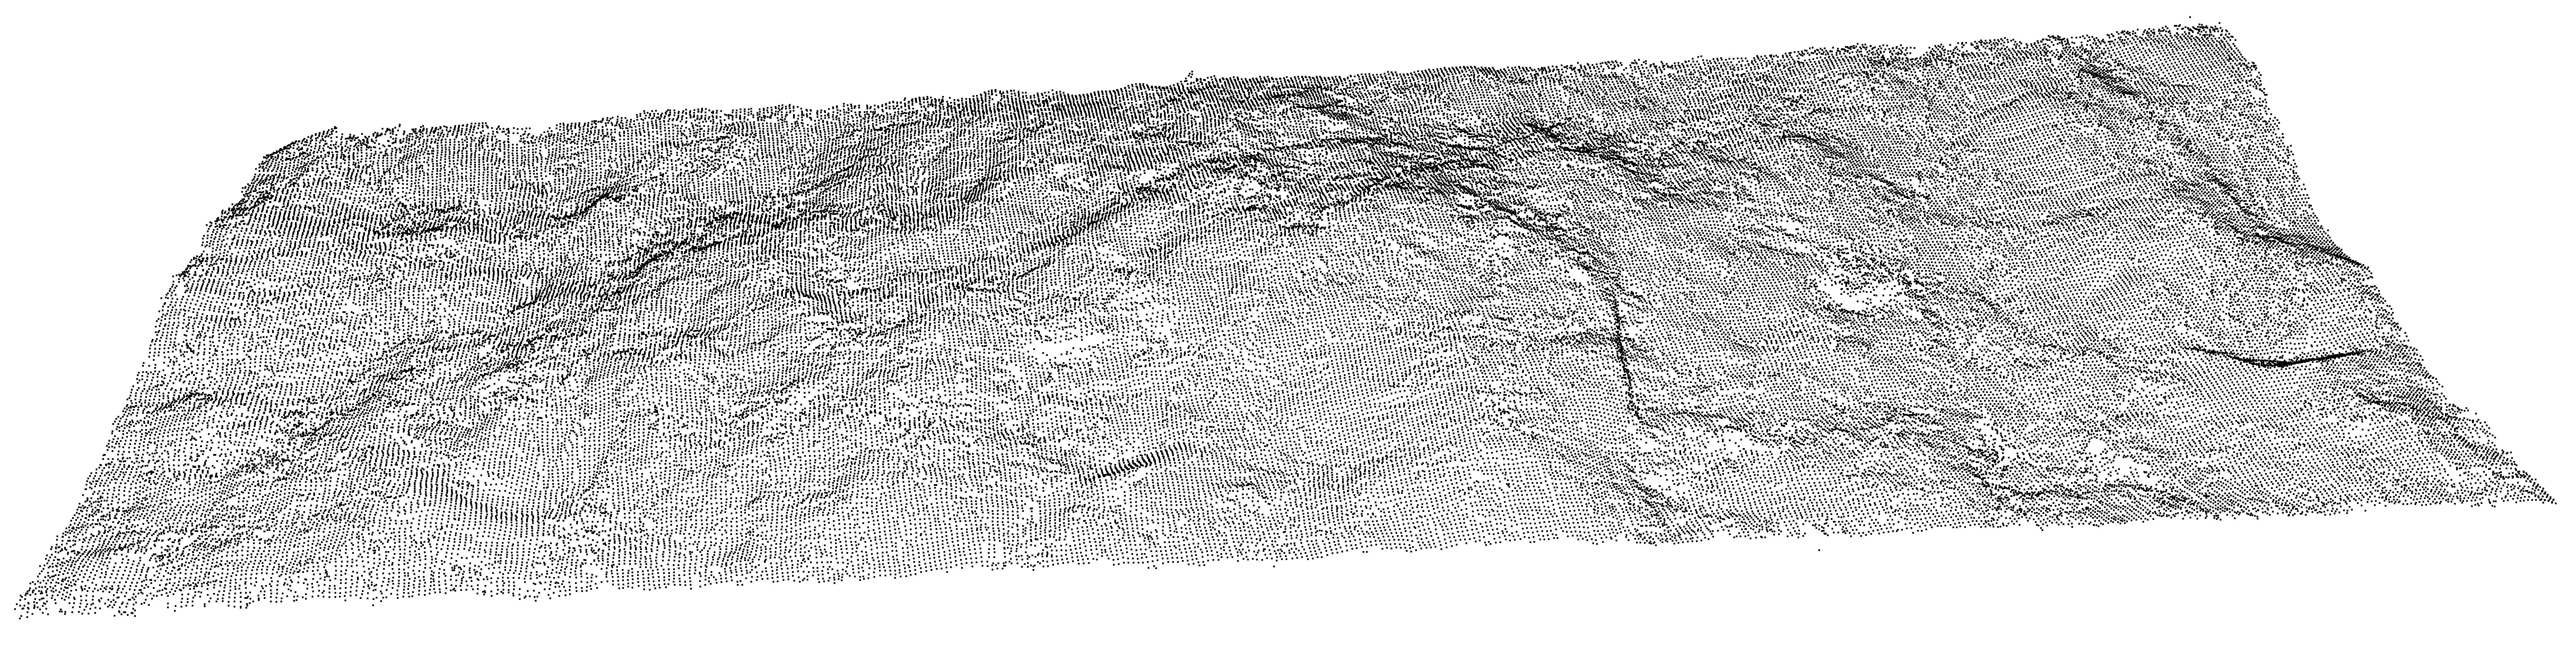
\includegraphics[width=0.7\textwidth]{./figures/MEX7_Point_cloud.png}
\end{center}
\caption{Point cloud representing the surface of a granite sample from Saxony. The size is 65 mm by 170 mm and the cloud contains approx. 98000 points. The shear direction is parallel to the long edge in a way that the shown surface remains in its position and its top counterpart is moved to the right.}
\label{fig:MEX7_pointCloud}
\end{figure}

Other basic laboratory tests are done to obtain rock parameters of the intact rock material like elastic constants, compressive strength, cohesion or friction angle. The values for the granite which was used in this model exercise can be found in table \ref{table:MEX7_rockParam}.

%\begin{table}
%\begin{center}
%\begin{tabular}{l c r r}
%variable & symbol & value & unit\\
%\hline
%density & $\rho$ & $2.59$ &$\text{g}/\text{cm}^3$\\
%compressive strength & $\sigma_c$ & $120.54$ &$\text{MPa}   $\\
%tensile strength & $\sigma_t$ & $7.02$&$ \text{MPa}   $\\
%elastic modulus & $E$ & $50.00$&$ \text{GPa}   $\\
%Poisson's ratio & $\nu$ & 0.26& \\
%fracture toughness & $K_I$ & $0.95$&$\text{MPa}\cdot\text{m}^{0.5}$\\
%friction angle & $\Phi$ &  $52.5$&$^\circ$\\
%cohesion & $c$ &  $22.5$&$ \text{MPa}   $\\
%\end{tabular}
%\caption{Rock parameters of the granite from Kirchberg, Saxony used in the %CNL direct shear test.}
%\label{table:MEX7_rockParam}
%\end{center}
%\end{table}

The shear test itself has been conducted for this model exercise using four different normal stress levels of $\sigma_n=1,2.5,5,7.5\,\text{MPa}$. After completing one level the parts were rearranged to their initial position and the next normal stress applied.

The task in this model exercise is to use the rock parameters from table \ref{table:MEX7_rockParam}, the geometry data of the point cloud and the boundary conditions of the direct shear test to back calculate the lab results. The whole data sets are provided as a download, see section \ref{DataManMex3-1CNL}. All research groups are invited to use this data to improve the quality of the calculations. The shown results will be provided as well to make it easy to compare different methodologies.
%------------------------------------------------------------------------------
\subsection{Model approach}
%------------------------------------------------------------------------------
A detailed description of the code can be found in the appendix.
%
The modelling of the direct shear tests is done by a self developed code using MATLAB. This includes the usage of matrices to represent the geometry of a rough surface. This is a simplification which speeds up the numerical process.
%
A function set does all the necessary steps from input through the calculations itself to the output. For comparison a couple of existing models where implemented as a reference.

\begin{itemize}
\item Barton-Bandis model \cite{BartonBandis1985}, which is widely used and due to its simplicity easy to understand.
\item Xia model \cite{Xia2014}, which uses quantitative roughness parameters with the drawback of complexity.
\item Casagrande algorithm \cite{Casagrande2017}, a semi analytical approach which was used for the algorithm development within the GeomInt project.
\end{itemize}

\begin{figure}[!ht]
\begin{center}
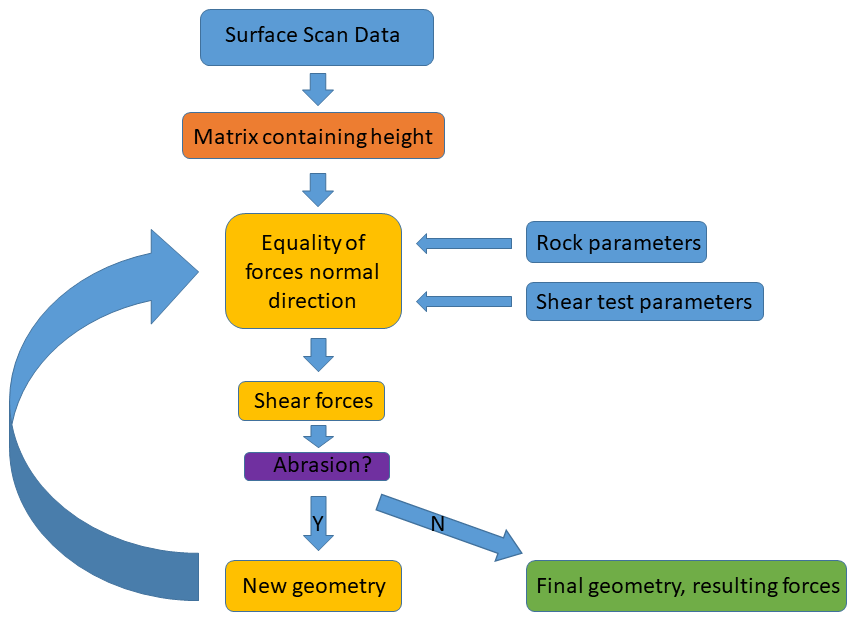
\includegraphics[width=0.5\textwidth]{./figures/MEX7_Scheme.png}
\end{center}
\caption{The functionality of the new model.}
\label{fig:MEX7_calculationScheme}
\end{figure}

A new algorithm was developed which uses the equality of normal forces as an approach to choose the surface elements which are in contact. The motivation is to make the calculation physically consistent. The scheme can be seen in Figure \ref{fig:MEX7_calculationScheme}. The shear forces are calculated using the approach of \cite{Casagrande2017}.
%------------------------------------------------------------------------------
\subsection{Results and discussion}
%------------------------------------------------------------------------------
The shear stress - shear displacement curves which result in lab testing have two values of main interest: The peak shear stress and the residual shear stress. A peak was just observed for the first shear stress level of $\sigma_n=1\,\text{MPa}$. In Figure \ref{fig:MEX7_Comparison_final_ME1_Peak} the results are shown. 

\begin{figure}[!ht]
\begin{center}
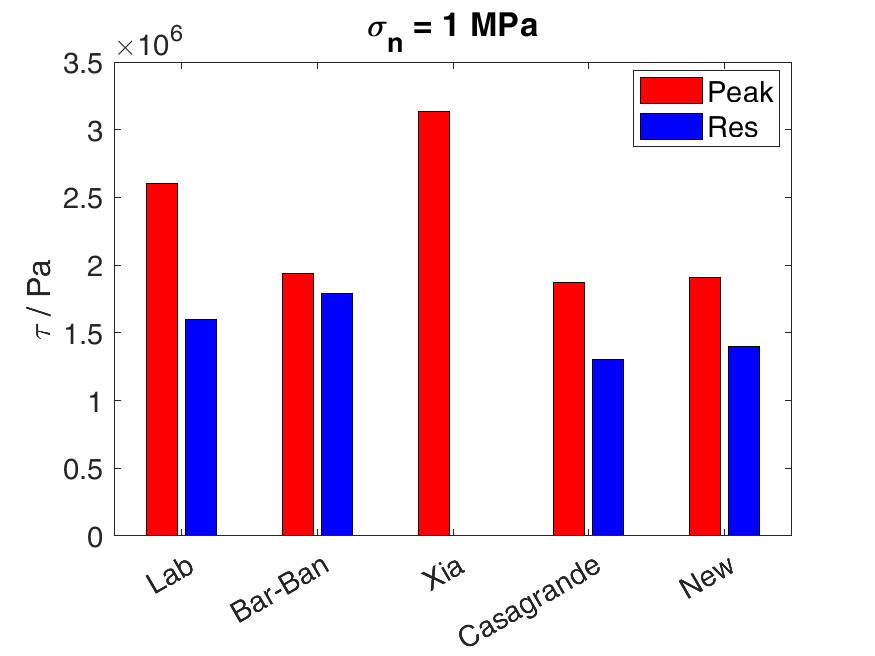
\includegraphics[width=0.8\textwidth]{./figures/MEX7_Comparison_final_Peak_Res_value_ME1.png}
\caption{Comparison of peak and residual shear strength for the first step of the shear test using different shear laws.}
\label{fig:MEX7_Comparison_final_ME1_Peak}
\end{center}
\end{figure}

At higher stress levels and due to the repeated shearing which causes wearing of the rock surface the curve shows no peak but a plateau which is the residual shear stress. The residual shear stress results for all stress levels are shown in Figure \ref{fig:MEX7_Comparison_final_ME1_Res}.

\begin{figure}[!ht]
\begin{center}
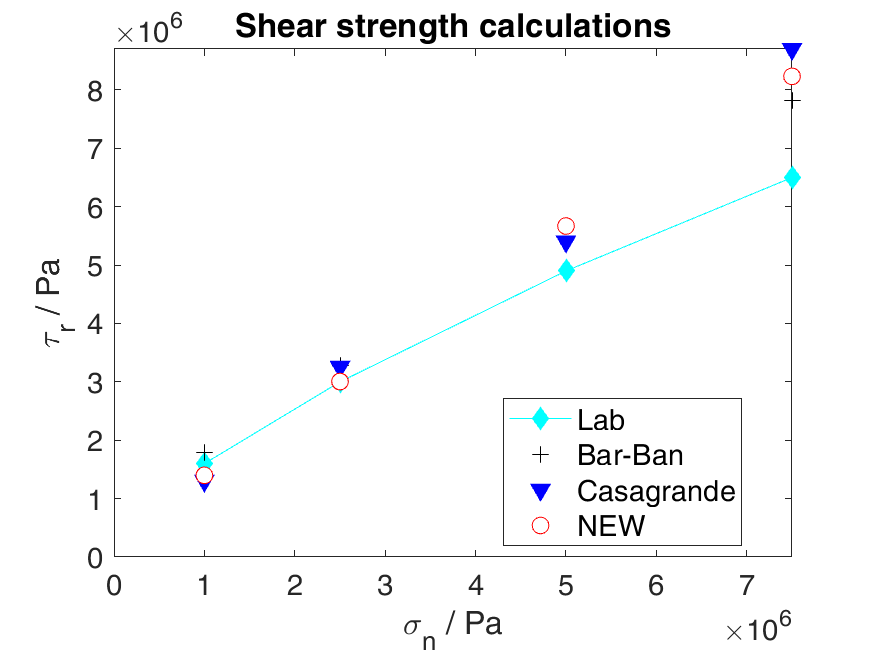
\includegraphics[width=0.8\textwidth]{./figures/MEX7_Comparison_final_res.png}
\caption{Comparison of residual shear strength using different shear laws.}
\label{fig:MEX7_Comparison_final_ME1_Res}
\end{center}
\end{figure}

The New shear law and the Barton-Bandis model allow to calculate complete shear curves. So for this models a comparison with the lab curves is possible and displayed in Figure \ref{fig:MEX7_New-Lab-BB}. 

\begin{figure}[!ht]
\begin{center}
\begin{tabular}{c c}
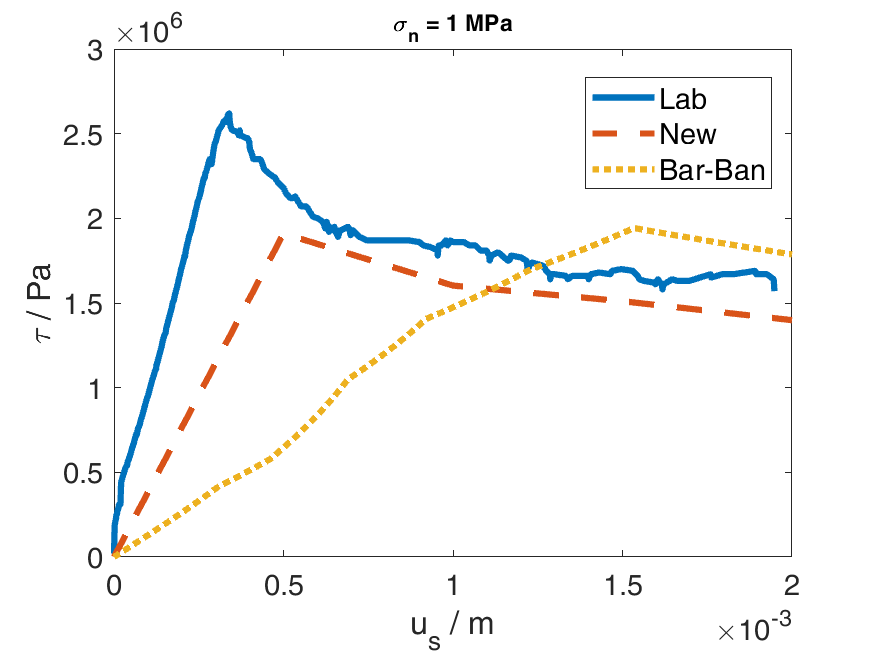
\includegraphics[width=0.45\textwidth]{./figures/MEX7_New-vs-Lab-vs-BB1.png} &
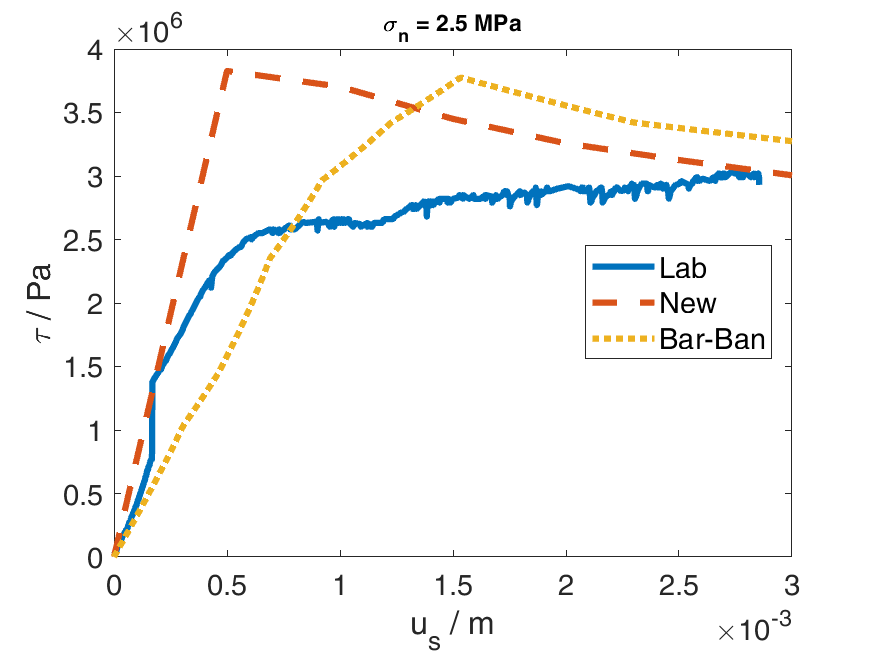
\includegraphics[width=0.45\textwidth]{./figures/MEX7_New-vs-Lab-vs-BB2.png} \\
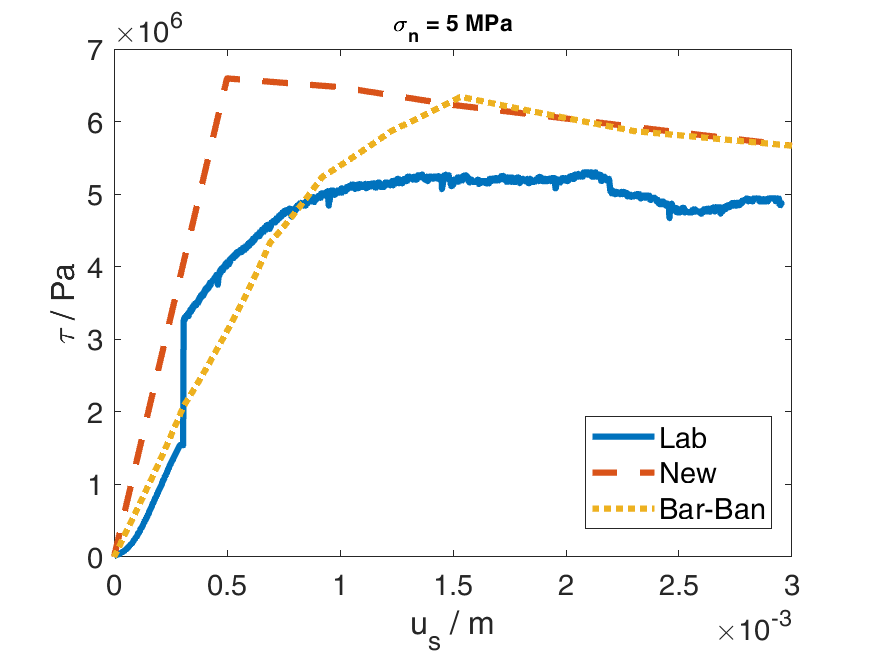
\includegraphics[width=0.45\textwidth]{./figures/MEX7_New-vs-Lab-vs-BB3.png} &
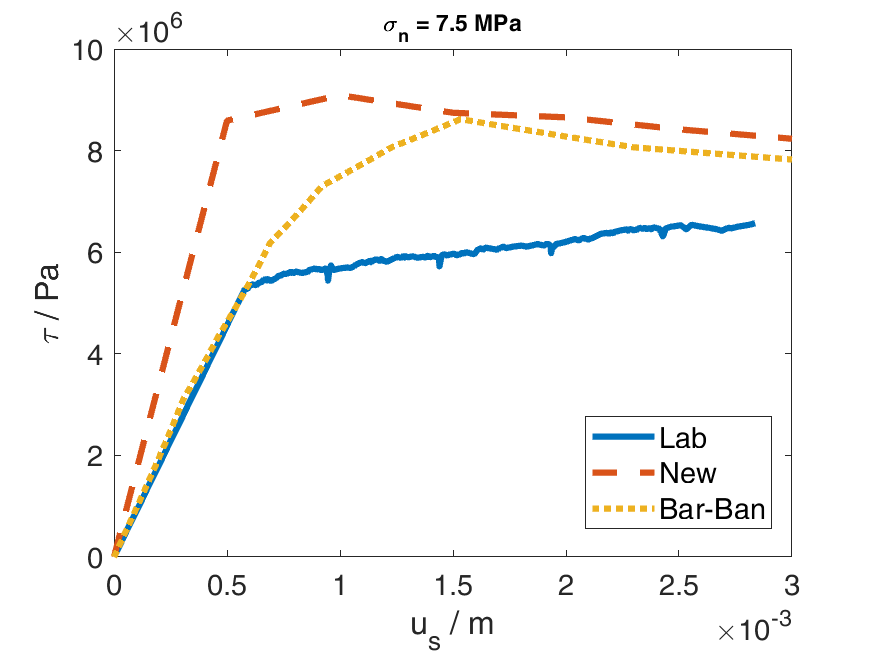
\includegraphics[width=0.45\textwidth]{./figures/MEX7_New-vs-Lab-vs-BB4.png}\\
\end{tabular}
\end{center}
\caption{Comparison of lab results with Barton-Bandis and New shear law for $\sigma_n=1,2.5,5,7.5\,\text{MPa}$ using a grid constant of $a=0.5\,\text{mm}$.}
\label{fig:MEX7_New-Lab-BB}
\end{figure}

\index{Barton-Bandis model}